% =====================================================================
%  MCMP117 -- Fundamentals of Operating Systems
%  Week 10 Course Notes: File & Directory Operations
%  Compile with XeLaTeX (twice):  xelatex MCMP117_Week10_Notes.tex
%  Needs ./figures/ and the ../code/ folder.
% =====================================================================
\documentclass[11pt,a4paper]{article}
\newcommand{\weeknum}{10}
% ---------- Page & fonts ---------------------------------------------
\usepackage[a4paper,margin=2.3cm,headheight=15pt]{geometry}
\usepackage{fontspec}
\IfFontExistsTF{Calibri}{\setmainfont{Calibri}}{\setmainfont{Carlito}}
\IfFontExistsTF{Cambria}{\newfontfamily\headfont{Cambria}}{\newfontfamily\headfont{Caladea}}
\IfFontExistsTF{Consolas}{\setmonofont[Scale=0.95]{Consolas}}{\setmonofont[Scale=0.88]{DejaVu Sans Mono}}
\usepackage{amsmath,amssymb}
\usepackage{microtype}
\linespread{1.12}
\setlength{\parskip}{0.55em}
\setlength{\parindent}{0pt}

% ---------- Colours (course design system) ----------------------------
\usepackage{xcolor}
\definecolor{dark}{HTML}{212121}
\definecolor{charcoal}{HTML}{36454F}
\definecolor{slate}{HTML}{50808E}
\definecolor{mint}{HTML}{02C39A}
\definecolor{mintdeep}{HTML}{028090}
\definecolor{light}{HTML}{F2F2F2}
\definecolor{muted}{HTML}{6B7679}

% ---------- Packages ---------------------------------------------------
\usepackage{graphicx}
\usepackage{float}
\usepackage{needspace}
\graphicspath{{figures/}}
\usepackage[font=small,labelfont={bf,color=mintdeep},justification=centering]{caption}
\usepackage{booktabs,longtable,array,tabularx}
\usepackage{enumitem}
\setlist{itemsep=0.25em,topsep=0.3em}
\usepackage{tikz}
\usetikzlibrary{arrows.meta,positioning,calc,shapes.geometric}
\usepackage{pgfplots}
\pgfplotsset{compat=1.17}
\usepackage[most]{tcolorbox}
\usepackage{titlesec}
\usepackage{fancyhdr}
\usepackage{xurl}
\usepackage[colorlinks=true,linkcolor=mintdeep,urlcolor=mintdeep,citecolor=mintdeep]{hyperref}

% ---------- Headings ----------------------------------------------------
\titleformat{\section}{\headfont\Large\bfseries\color{charcoal}}{\color{mint}\thesection}{0.7em}{}
\titleformat{\subsection}{\headfont\large\bfseries\color{charcoal}}{\color{mintdeep}\thesubsection}{0.6em}{}
\titleformat{\subsubsection}{\headfont\normalsize\bfseries\color{mintdeep}}{}{0em}{}
\titlespacing*{\section}{0pt}{1.6em}{0.6em}
\titlespacing*{\subsection}{0pt}{1.2em}{0.4em}

% ---------- Header / footer -----------------------------------------------
\pagestyle{fancy}
\fancyhf{}
\fancyhead[L]{\small\color{muted}MCMP117 --- Fundamentals of Operating Systems}
\fancyhead[R]{\small\color{muted}Week \weeknum{} Notes}
\fancyfoot[C]{\small\color{muted}\thepage}
\renewcommand{\headrulewidth}{0pt}

% ---------- Boxes ---------------------------------------------------------
\newtcolorbox{keyidea}[1][Key idea]{enhanced,breakable,colback=charcoal,colframe=charcoal,
  coltext=white,fonttitle=\headfont\bfseries\color{mint},title={#1},
  attach title to upper={\par\smallskip},boxrule=0pt,arc=3pt,left=10pt,right=10pt,top=8pt,bottom=8pt}
\newtcolorbox{example}[1][Worked example]{enhanced,colback=light,colframe=light,
  fonttitle=\headfont\bfseries\color{mintdeep},title={#1},attach title to upper={\par\smallskip},
  boxrule=0pt,arc=3pt,left=10pt,right=10pt,top=8pt,bottom=8pt}
\newtcolorbox{tryit}[1][Try it yourself]{enhanced,breakable,colback=white,colframe=mint,
  fonttitle=\headfont\bfseries\color{mintdeep},title={#1},attach title to upper={\par\smallskip},
  boxrule=0.8pt,arc=3pt,left=10pt,right=10pt,top=8pt,bottom=8pt}
\newtcolorbox{histnote}[1][Historical note]{enhanced,breakable,colback=white,colframe=slate!40,
  fonttitle=\headfont\bfseries\color{slate},title={#1},attach title to upper={\par\smallskip},
  boxrule=0.5pt,arc=3pt,left=10pt,right=10pt,top=8pt,bottom=8pt,fontupper=\small}

% Photo helper: fits image inside a box, never distorted (keepaspectratio)
\newcommand{\photo}[3]{\includegraphics[width=#1,height=#2,keepaspectratio]{#3}}

\newcommand{\term}[1]{\textbf{\color{mintdeep}#1}}
\newcommand{\cmd}[1]{\texttt{#1}}


% ---------- Code listings ----------------------------------------------------
\usepackage{listings}
\lstdefinestyle{course}{
  basicstyle=\ttfamily\small, columns=fullflexible, keepspaces=true,
  backgroundcolor=\color{dark}, rulecolor=\color{dark}, frame=single, framesep=6pt,
  xleftmargin=8pt, xrightmargin=8pt, aboveskip=0.8em, belowskip=0.6em,
  basicstyle=\ttfamily\small\color{light},
  keywordstyle=\color{mint}\bfseries, commentstyle=\color{white!60}\itshape,
  stringstyle=\color{orange!70!yellow}, numberstyle=\tiny\color{muted},
  numbers=left, numbersep=10pt, showstringspaces=false, breaklines=true,
  tabsize=4, upquote=true}
\lstdefinestyle{term}{style=course, numbers=none, keywordstyle=\color{light},
  commentstyle=\color{white!60}, stringstyle=\color{light}}
\lstset{style=course,language=C}
\usepackage{textcomp}

\begin{document}
% ============================ Week 10 body ============================
% Terminal listings in this practical week are long: use a slightly smaller font.
\lstdefinestyle{term}{style=course, numbers=none, keywordstyle=\color{light},
  commentstyle=\color{white!60}, stringstyle=\color{light},
  basicstyle=\ttfamily\footnotesize\color{light}, aboveskip=0.5em, belowskip=0.4em,
  escapeinside={<@}{@>}}
\setlength{\parskip}{0.45em}
\thispagestyle{empty}
\begin{tcolorbox}[enhanced,colback=dark,colframe=dark,arc=0pt,boxrule=0pt,
  left=18pt,right=18pt,top=20pt,bottom=20pt,coltext=white]
{\small\color{mint}\textsc{MCMP117 \,·\, Week 10 \,·\, Course Notes}}\par\medskip
{\headfont\fontsize{26}{30}\selectfont\bfseries Fundamentals of Operating Systems}\par\medskip
{\large File \& Directory Operations}\par\smallskip
{\small\itshape\color{white!70} Create, copy, move, delete, view and link files --- and know what the kernel does each time.}
\end{tcolorbox}

\vspace{0.4em}
{\small
\textbf{Instructor:} Asst.\ Prof.\ Dr.\ (Ph.D.) Hasan Oğuz\\
Head of the Electronical Communication Technology Programme, Vocational School\\
Istanbul Okan University\par}

\vspace{0.8em}
\begin{keyidea}[What you should be able to do after this week]
\begin{enumerate}[leftmargin=1.4em]
  \item Explain, in terms of directory entries, inodes and data blocks (Week~7), what \cmd{touch}, \cmd{cp}, \cmd{mv}, \cmd{ln}, \cmd{ln -s} and \cmd{rm} change.
  \item Create directories and files with \cmd{mkdir} (\cmd{-p}) and \cmd{touch}, and read the three timestamps atime, mtime and ctime.
  \item Copy, move, rename and delete files and directory trees with \cmd{cp}, \cmd{mv}, \cmd{rm}, \cmd{rmdir} --- safely.
  \item Use the wildcards \texttt{*}, \texttt{?}, \texttt{[\,]} and brace expansion \texttt{\{a,b\}}, \texttt{\{1..5\}}, and explain that the \emph{shell} expands them.
  \item Work with file names that contain spaces.
  \item Inspect files with \cmd{cat}, \cmd{less}, \cmd{head}, \cmd{tail}, \cmd{wc}, \cmd{file}, \cmd{stat}, \cmd{du} and \cmd{df}.
  \item Create hard and symbolic links and predict what happens when the original is deleted.
\end{enumerate}
\end{keyidea}

\setcounter{tocdepth}{1}
\tableofcontents

% =====================================================================
\section{From Week 9 to Week 10}

In Week~9 we met the terminal and the shell, learned the anatomy of a command (\texttt{command}\ \texttt{-options}\ \texttt{arguments}), and moved around the Linux directory tree with \cmd{pwd}, \cmd{ls} and \cmd{cd}, using absolute paths (\texttt{/home/\allowbreak student/\allowbreak lab}) and relative paths (\texttt{docs}, \texttt{../data}). We only \emph{looked}. This week we \emph{change} the file system: we create, copy, move, rename, delete and link files and directories, and we look inside them.

Everything here rests on the file-system theory of Week~7, so we start with a short recap. Then come the commands, each shown with real output.

\subsection*{Setting up}

All examples run in the practice folder created by the lab script (it is in the \cmd{code/} folder of every Linux week). Run it before each session; it deletes and re-creates \emph{only} \texttt{\textasciitilde/lab}:
\begin{lstlisting}[style=term]
$ bash ~/mcmp117_lab_setup.sh
$ cd ~/lab
\end{lstlisting}
Every demo of the slides is a script in \cmd{code/} (for example \cmd{demo\_cp\_mv.sh}) and its captured output is the matching \cmd{out\_*.txt} file. The prompt \texttt{student@okan-lab:\textasciitilde/lab\$} shows the user, the machine and the current directory; you type only what follows the \texttt{\$}.

\begin{keyidea}[Your output will differ slightly]
The outputs were captured as the ordinary user \texttt{student} with \texttt{LC\_ALL=C.UTF-8}. In other locales \cmd{ls} may \emph{sort} differently (in the C locale capitals come first, so \texttt{IMG\_014.JPG} is listed before \texttt{holiday.jpeg}). Dates, times (ours are in UTC, \texttt{+0000}; in Türkiye you will see \texttt{+0300}), inode numbers, disk sizes and user IDs will be different on your machine. Everything else should match.
\end{keyidea}

% =====================================================================
\section{Names, Inodes and System Calls}
\label{sec:inodes}

\subsection{Recap: what is stored where}

Remember from Week~7: a \term{directory} is a table of (name, inode number) pairs. The \term{inode} holds everything else about a file --- type, size, owner, permissions, timestamps, \term{link count} and the pointers to the \term{data blocks} --- but \emph{not} its name. That is why one inode can have several names, and why some operations are instant while others copy data.

\begin{figure}[H]
\centering
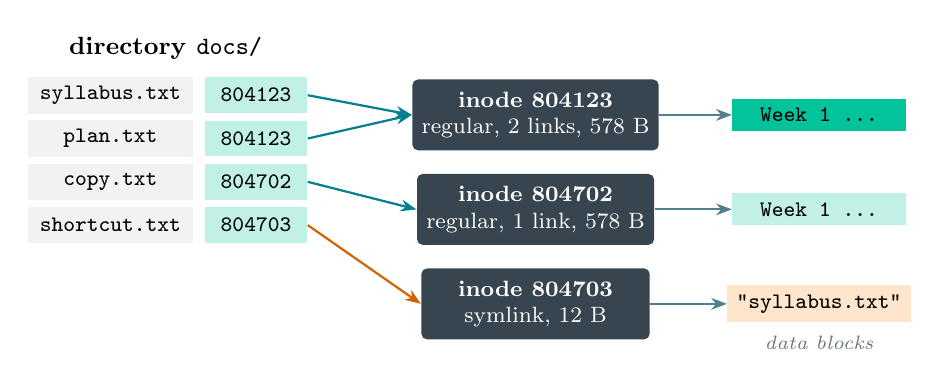
\begin{tikzpicture}[e/.style={rectangle,fill=light,minimum height=0.45cm,font=\footnotesize\ttfamily},
  ino/.style={rectangle,rounded corners=2pt,fill=charcoal,text=white,align=center,font=\footnotesize,minimum width=2.9cm,minimum height=0.9cm},
  arr/.style={-{Stealth[length=2mm]},thick,mintdeep}]
\node[font=\small\bfseries] at (1.3,0.6) {directory \texttt{docs/}};
\foreach \n/\i [count=\k from 0] in {syllabus.txt/804123,plan.txt/804123,copy.txt/804702,shortcut.txt/804703} {
  \node[e,minimum width=2.1cm] at (0.6,-0.55*\k) {\n};
  \node[e,minimum width=1.3cm,fill=mint!25] (d\k) at (2.45,-0.55*\k) {\i};
}
\node[ino] (A) at (6.0,-0.25) {\textbf{inode 804123}\\regular, 2 links, 578 B};
\node[ino] (B) at (6.0,-1.45) {\textbf{inode 804702}\\regular, 1 link, 578 B};
\node[ino] (Cn) at (6.0,-2.65) {\textbf{inode 804703}\\symlink, 12 B};
\draw[arr] (d0.east) -- (A.west); \draw[arr] (d1.east) -- (A.west);
\draw[arr] (d2.east) -- (B.west); \draw[arr,orange!80!black] (d3.east) -- (Cn.west);
\node[rectangle,fill=mint,font=\footnotesize\ttfamily,minimum width=2.2cm] (a) at (9.6,-0.25) {Week 1 \dots};
\node[rectangle,fill=mint!25,font=\footnotesize\ttfamily,minimum width=2.2cm] (b) at (9.6,-1.45) {Week 1 \dots};
\node[rectangle,fill=orange!20,font=\footnotesize\ttfamily,minimum width=2.2cm] (c) at (9.6,-2.65) {"syllabus.txt"};
\draw[arr,slate] (A) -- (a); \draw[arr,slate] (B) -- (b); \draw[arr,slate] (Cn) -- (c);
\node[font=\scriptsize\itshape,text=muted] at (9.6,-3.15) {data blocks};
\end{tikzpicture}
\caption{Real situation from the links demo (Section~\ref{sec:links}): \texttt{plan.txt} is a hard link, \texttt{copy.txt} a copy, \texttt{shortcut.txt} a symbolic link.}
\label{fig:inodes}
\end{figure}

With this picture every command of the week can be described by \emph{what it changes}:

\begin{center}
\renewcommand{\arraystretch}{1.25}
\begin{tabularx}{\linewidth}{>{\ttfamily}l >{\raggedright\arraybackslash}X >{\ttfamily}l}
\toprule
\textrm{\textbf{Command}} & \textbf{What changes} & \textrm{\textbf{System call}} \\
\midrule
touch new & a new name and a new (empty) inode & openat(O\_CREAT) \\
mkdir d & a new name and a new directory inode & mkdir() \\
cp a b & a new name, a new inode \emph{and} a copy of all data & open/read/write \\
mv a b & only directory entries; same inode, data untouched & renameat2() \\
ln a b & a new name pointing to the \emph{same} inode; link count $+1$ & linkat() \\
ln -s a b & a new name and a small inode whose data is the path \texttt{a} & symlinkat() \\
rm a & a name is removed; link count $-1$; data freed at $0$ & unlinkat() \\
rmdir d & an empty directory is removed & rmdir() \\
\bottomrule
\end{tabularx}
\end{center}

\subsection{Commands are programs; their work is done by system calls}

Each command is a small program in \texttt{/usr/bin}. The shell starts it with \cmd{fork()} and \cmd{exec()} (Week~3), and the program asks the kernel to do the real work through a \term{system call} (Week~2). With \cmd{strace} we can watch this; \cmd{-e trace=\dots} shows only the calls we name (script \cmd{demo\_strace.sh}; the lines \texttt{+++ exited with 0 +++} after each command are omitted):

\begin{lstlisting}[style=term]
student@okan-lab:~/lab$ strace -e trace=mkdir,mkdirat mkdir newdir
mkdir("newdir", 0777)                   = 0
student@okan-lab:~/lab$ strace -e trace=rename,renameat,renameat2 mv newdir olddir
renameat2(AT_FDCWD, "newdir", AT_FDCWD, "olddir", RENAME_NOREPLACE) = 0
student@okan-lab:~/lab$ touch file1
student@okan-lab:~/lab$ strace -e trace=link,linkat ln file1 file2
linkat(AT_FDCWD, "file1", AT_FDCWD, "file2", 0) = 0
student@okan-lab:~/lab$ strace -e trace=symlink,symlinkat ln -s olddir sym
symlinkat("olddir", AT_FDCWD, "sym")    = 0
student@okan-lab:~/lab$ strace -e trace=unlink,unlinkat rm file1 file2 sym
unlinkat(AT_FDCWD, "file1", 0)          = 0
unlinkat(AT_FDCWD, "file2", 0)          = 0
unlinkat(AT_FDCWD, "sym", 0)            = 0
student@okan-lab:~/lab$ strace -e trace=rmdir,unlinkat rmdir olddir
rmdir("olddir")                         = 0
\end{lstlisting}

Observe:
\begin{itemize}
  \item \cmd{mv} did not copy a single byte: it made one \cmd{renameat2()} call. The flag \texttt{RENAME\_NOREPLACE} means ``fail if the target exists''; \cmd{mv} uses it first and only replaces a target deliberately.
  \item \cmd{rm} with three names makes three \cmd{unlinkat()} calls. The kernel's name for deleting is \emph{unlink}: it removes one \emph{link} (name) of an inode.
  \item The \texttt{\dots at} versions take a directory as their first argument; \texttt{AT\_FDCWD} means ``relative to the current working directory'' --- exactly the relative paths of Week~9.
\end{itemize}

% =====================================================================
\section{Creating: \texttt{mkdir} and \texttt{touch}}

\subsection{\texttt{mkdir}: make directories}

\cmd{mkdir name} creates one empty directory. Two errors are common: the name is already taken, or a \emph{parent} directory on the path does not exist. The option \cmd{-p} (\emph{parents}) creates every missing directory on the path and is silent if the directory already exists (\cmd{demo\_mkdir\_touch.sh}):

\begin{lstlisting}[style=term]
student@okan-lab:~/lab$ mkdir test
student@okan-lab:~/lab$ ls -ld test
drwxrwxr-x 2 student student 4096 Oct 12 08:47 test
student@okan-lab:~/lab$ mkdir test
mkdir: cannot create directory <@‘@>test<@’@>: File exists
student@okan-lab:~/lab$ mkdir trip/day1
mkdir: cannot create directory <@‘@>trip/day1<@’@>: No such file or directory
student@okan-lab:~/lab$ mkdir -p trip/day1
student@okan-lab:~/lab$ mkdir -p work/2026/october
student@okan-lab:~/lab$ tree work trip
work
<@└──@> 2026
    <@└──@> october
trip
<@└──@> day1

5 directories, 0 files
\end{lstlisting}

\cmd{ls -ld test} lists the directory \emph{itself} (\cmd{-d}), not its contents. Its link count is $2$: the name \texttt{test} in \texttt{\textasciitilde/lab} and the entry \texttt{.} inside it. \cmd{tree} draws a directory tree; its final count includes the starting directories ($5$: \texttt{work}, \texttt{2026}, \texttt{october}, \texttt{trip}, \texttt{day1}).

\subsection{\texttt{touch}: empty files and timestamps}

\cmd{touch file} has two effects. If the file does not exist, it is created with size $0$. If it exists, its content is left alone and only its timestamps are set to ``now''. With \cmd{-d} you can set any time:

\begin{lstlisting}[style=term]
student@okan-lab:~/lab$ touch todo.txt
student@okan-lab:~/lab$ ls -l todo.txt
-rw-rw-r-- 1 student student 0 Oct 12 08:47 todo.txt
student@okan-lab:~/lab$ touch -d "2026-01-15 09:30" todo.txt
student@okan-lab:~/lab$ ls -l todo.txt
-rw-rw-r-- 1 student student 0 Jan 15  2026 todo.txt
student@okan-lab:~/lab$ stat todo.txt
  File: todo.txt
  Size: 0               Blocks: 0          IO Block: 4096   regular empty file
Device: 254,0   Inode: 804708      Links: 1
Access: (0664/-rw-rw-r--)  Uid: ( 1010/ student)   Gid: ( 1012/ student)
Access: 2026-01-15 09:30:00.000000000 +0000
Modify: 2026-01-15 09:30:00.000000000 +0000
Change: 2026-10-12 08:47:56.442757013 +0000
 Birth: 2026-10-12 08:47:56.430757013 +0000
student@okan-lab:~/lab$ touch todo.txt
student@okan-lab:~/lab$ ls -l todo.txt
-rw-rw-r-- 1 student student 0 Oct 12 08:47 todo.txt
\end{lstlisting}

Note that \cmd{ls -l} shows \texttt{Jan 15\ \ 2026} --- a year instead of a time of day --- because the date is more than six months away from today. \cmd{stat} (Section~\ref{sec:stat}) shows all four times kept in the inode.

\subsection{Three (or four) timestamps}

An inode keeps three times: \term{atime} (Access, last read of the data), \term{mtime} (Modify, last change of the data --- the time \cmd{ls -l} shows) and \term{ctime} (Change, last change of the \emph{inode}: data, link count, permissions, owner, times). \textbf{ctime is not the creation time}; newer file systems such as ext4 also record a creation time, shown by \cmd{stat} as \emph{Birth}.

We verified on our test machine (ext4) which action changes which time:

\begin{center}
\renewcommand{\arraystretch}{1.2}
\begin{tabular}{@{}llll@{}}
\toprule
\textbf{Action} & \textbf{atime} & \textbf{mtime} & \textbf{ctime} \\
\midrule
read: \cmd{cat f} & yes (lazily) & --- & --- \\
write: \cmd{echo x >> f} & --- & yes & yes \\
\cmd{touch f} & yes & yes & yes \\
rename: \cmd{mv f g} & --- & --- & yes \\
new hard link: \cmd{ln f h} & --- & --- & yes \\
permissions: \cmd{chmod} (Week~11) & --- & --- & yes \\
\bottomrule
\end{tabular}
\end{center}

``Lazily'': to avoid a disk write for every read, Linux mounts file systems with \texttt{relatime} and updates atime only when it is older than mtime or more than $24$~hours old. Backup programs and \cmd{make} rely on mtime; \cmd{cp -p} keeps the original mtime of a file instead of giving the copy the current time.

% =====================================================================
\section{Copying, Moving and Deleting}

\subsection{\texttt{cp}: copy}

\cmd{cp SOURCE TARGET} copies a file. If \texttt{TARGET} is an existing directory, the copy keeps its name and goes inside it; otherwise \texttt{TARGET} is the new name. With several sources, the last argument must be a directory. Options: \cmd{-v} (verbose) reports each copy, \cmd{-i} (interactive) asks before overwriting, \cmd{-r} (recursive) copies directories (\cmd{demo\_cp\_mv.sh}):

\begin{lstlisting}[style=term]
student@okan-lab:~/lab$ cp docs/syllabus.txt backup/
student@okan-lab:~/lab$ cp docs/syllabus.txt backup/syllabus_copy.txt
student@okan-lab:~/lab$ ls backup
syllabus.txt  syllabus_copy.txt
student@okan-lab:~/lab$ cp -v docs/notes_01.txt docs/notes_02.txt backup/
'docs/notes_01.txt' -> 'backup/notes_01.txt'
'docs/notes_02.txt' -> 'backup/notes_02.txt'
student@okan-lab:~/lab$ cp -i docs/syllabus.txt backup/
cp: overwrite 'backup/syllabus.txt'? n
student@okan-lab:~/lab$ cp projects/alpha backup/
cp: -r not specified; omitting directory 'projects/alpha'
student@okan-lab:~/lab$ cp -r projects/alpha backup/
student@okan-lab:~/lab$ tree backup
backup
<@├──@> alpha
<@│  @> <@├──@> README.md
<@│  @> <@├──@> docs
<@│  @> <@│  @> <@└──@> design.txt
<@│  @> <@└──@> src
<@│  @>     <@└──@> main.c
<@├──@> notes_01.txt
<@├──@> notes_02.txt
<@├──@> syllabus.txt
<@└──@> syllabus_copy.txt

4 directories, 7 files
student@okan-lab:~/lab$ ls -i docs/syllabus.txt backup/syllabus.txt
804330 backup/syllabus.txt  804123 docs/syllabus.txt
\end{lstlisting}

Observations:
\begin{itemize}
  \item \cmd{cp -i} asked before overwriting; we answered \texttt{n}. (In the script the answer is supplied by \cmd{echo n}; in a terminal you type it.) \textbf{Without} \cmd{-i}, \cmd{cp} overwrites an existing file silently.
  \item A directory is not copied without \cmd{-r}. \emph{Recursive} means: copy the directory, then do the same for every entry in it, and so on down the tree.
  \item \cmd{ls -i} shows \emph{different} inode numbers ($804330$ and $804123$): a copy is a new, independent file. Changing one does not change the other.
\end{itemize}
Useful extras: \cmd{cp -p} also keeps times and permissions; \cmd{cp -a} (archive) is \cmd{-r} plus everything that \cmd{-p} keeps, and is what you want for backups.

\begin{tryit}[A silent trap]
If \texttt{backup/} does \emph{not} exist, \cmd{cp notes.txt backup} creates a \emph{file} named \texttt{backup}. Writing \texttt{backup/} with a trailing slash makes \cmd{cp} fail with an error instead.
\end{tryit}

\subsection{\texttt{mv}: rename and move}

Linux has no separate rename command for single files: \cmd{mv} does both. Inside one directory \cmd{mv old new} renames; \cmd{mv file dir/} moves the name into another directory. Directories are moved the same way, without \cmd{-r}:

\begin{lstlisting}[style=term]
student@okan-lab:~/lab$ mv backup/syllabus.txt backup/syllabus_old.txt
student@okan-lab:~/lab$ ls -i backup/syllabus_old.txt
804330 backup/syllabus_old.txt
student@okan-lab:~/lab$ mv -v docs/notes_03.txt backup/
renamed 'docs/notes_03.txt' -> 'backup/notes_03.txt'
student@okan-lab:~/lab$ mv backup/alpha backup/alpha_2026
student@okan-lab:~/lab$ ls docs backup
backup:
alpha_2026    notes_02.txt  syllabus_copy.txt
notes_01.txt  notes_03.txt  syllabus_old.txt

docs:
'final report.txt'   notes_01.txt   syllabus.txt
 linux_quotes.txt    notes_02.txt
\end{lstlisting}

The inode number of \texttt{backup/syllabus.txt} was $804330$ before the rename and is still $804330$ after it: only the directory entry changed (one \cmd{renameat2()} call, Section~\ref{sec:inodes}). Hence \cmd{mv} within one file system is instant whatever the file size. Between two file systems (for example from the disk to a USB stick) the inode cannot move, so \cmd{mv} copies the data and then deletes the original. Like \cmd{cp}, \cmd{mv} overwrites an existing target silently; use \cmd{mv -i}.

\subsection{\texttt{rm} and \texttt{rmdir}: delete}

\cmd{rm} removes names; \cmd{rmdir} removes \emph{empty} directories (\cmd{demo\_rm.sh}):

\begin{lstlisting}[style=term]
student@okan-lab:~/lab$ touch junk1.txt junk2.txt junk3.txt
student@okan-lab:~/lab$ rm junk1.txt
student@okan-lab:~/lab$ rm -i junk2.txt
rm: remove regular empty file 'junk2.txt'? y
student@okan-lab:~/lab$ rm -v junk3.txt
removed 'junk3.txt'
student@okan-lab:~/lab$ ls junk*
ls: cannot access 'junk*': No such file or directory
student@okan-lab:~/lab$ mkdir empty_dir
student@okan-lab:~/lab$ rmdir empty_dir
student@okan-lab:~/lab$ rmdir projects/beta
rmdir: failed to remove 'projects/beta': Directory not empty
student@okan-lab:~/lab$ rm projects/beta
rm: cannot remove 'projects/beta': Is a directory
student@okan-lab:~/lab$ cp -r projects/beta beta_copy
student@okan-lab:~/lab$ tree beta_copy
...
3 directories, 3 files
student@okan-lab:~/lab$ rm -rv beta_copy
removed 'beta_copy/src/main.c'
removed directory 'beta_copy/src'
removed 'beta_copy/README.md'
removed 'beta_copy/docs/design.txt'
removed directory 'beta_copy/docs'
removed directory 'beta_copy'
student@okan-lab:~/lab$ ls
README.txt  backup  data  docs  logs  photos  projects  scripts  src
\end{lstlisting}

\begin{itemize}
  \item \cmd{rm junk1.txt} prints nothing and asks nothing.
  \item \cmd{rm -i} asks (``remove regular empty file?''); \cmd{rm -v} reports what it removed.
  \item \cmd{ls junk*} fails because no name matches the pattern any more; the shell then passes the pattern unchanged (Section~\ref{sec:glob}).
  \item \cmd{rmdir} refuses a non-empty directory; \cmd{rm} without \cmd{-r} refuses any directory.
  \item \cmd{rm -rv} shows the order of work: every directory is emptied first, because the kernel's \cmd{rmdir()} only removes empty directories.
\end{itemize}

\begin{keyidea}[Warning: rm is forever]
There is \textbf{no recycle bin} on the command line. \cmd{rm} calls \cmd{unlinkat()}; when the link count reaches $0$ (and no program has the file open) the blocks are marked free and soon reused. The ``Trash'' of a desktop is a feature of the file manager, not of the kernel.
\begin{itemize}
  \item Before \cmd{rm} with a pattern, run \cmd{ls} with the \emph{same} pattern; check where you are with \cmd{pwd}.
  \item \cmd{rm -r} deletes a whole tree. A stray space is enough for disaster: \cmd{rm -r \textasciitilde/lab /old} deletes \texttt{\textasciitilde/lab} \emph{and} tries \texttt{/old}.
  \item \cmd{rm -f} (force) never asks and hides errors. Never run \cmd{rm -rf} with \cmd{sudo} (Week~11) unless you understand every character.
\end{itemize}
If you damage \texttt{\textasciitilde/lab}, just run the setup script again. On a real system, backups are the only undo.
\end{keyidea}

% =====================================================================
\section{Wildcards and Brace Expansion}
\label{sec:glob}

\subsection{Who expands \texttt{*}? The shell}

When you type \cmd{ls *.jpg}, the program \cmd{ls} never sees the star. \emph{Before} starting the command, bash reads the current directory, finds all names that match the pattern, sorts them, and puts them on the command line as separate arguments. This is called \term{globbing} (pathname expansion). Then \cmd{fork()} and \cmd{exec()} start \cmd{ls} with the finished list (Week~3).

\begin{figure}[H]
\centering
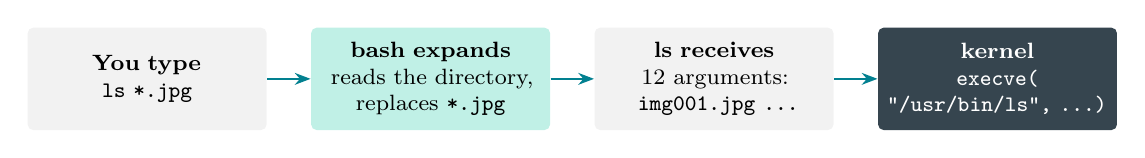
\begin{tikzpicture}[b/.style={rectangle,rounded corners=2pt,minimum width=3.0cm,minimum height=1.3cm,align=center,font=\footnotesize,text width=2.8cm},
  arr/.style={-{Stealth[length=2mm]},thick,mintdeep}]
\node[b,fill=light] (u) at (0,0) {\textbf{You type}\\\texttt{ls *.jpg}};
\node[b,fill=mint!25] (s) at (3.6,0) {\textbf{bash expands}\\reads the directory, replaces \texttt{*.jpg}};
\node[b,fill=light] (l) at (7.2,0) {\textbf{ls receives}\\12 arguments:\\\texttt{img001.jpg \dots}};
\node[b,fill=charcoal,text=white] (k) at (10.8,0) {\textbf{kernel}\\\texttt{execve(}\\\texttt{"/usr/bin/ls", \dots)}};
\draw[arr] (u) -- (s); \draw[arr] (s) -- (l); \draw[arr] (l) -- (k);
\end{tikzpicture}
\caption{Wildcards are expanded by the shell, not by the command.}
\end{figure}

Three consequences:
\begin{enumerate}[leftmargin=1.4em]
  \item \cmd{echo} shows exactly what a command will receive, so it is the perfect tool to test a pattern.
  \item Every command ``supports'' wildcards, because no command ever sees them.
  \item If nothing matches, bash leaves the pattern unchanged; the command then looks for a file literally named \texttt{junk*} and reports that it does not exist.
\end{enumerate}

\subsection{The patterns}

\begin{center}
\renewcommand{\arraystretch}{1.25}
\begin{tabularx}{\linewidth}{>{\ttfamily}l >{\raggedright\arraybackslash}X >{\ttfamily}l >{\raggedright\arraybackslash}X}
\toprule
\textrm{\textbf{Pattern}} & \textbf{Matches} & \textrm{\textbf{Example}} & \textbf{Result in \texttt{photos/}} \\
\midrule
* & any string, also the empty one & *.jpg & $12$ names, img001--img012 \\
? & exactly one character & img00?.jpg & $9$ names, img001--img009 \\
{[0-2]} & one character from a range & img01[0-2].jpg & img010, img011, img012 \\
{[135]} & one of the listed characters & img00[135].jpg & img001, img003, img005 \\
{[!0]} & one character \emph{not} in the set & img0[!0]* & img010 \dots\ img013 \\
\bottomrule
\end{tabularx}
\end{center}

Two rules: Linux names are \emph{case-sensitive} (\texttt{*.jpg} does not match \texttt{IMG\_014.JPG}), and \texttt{*} does not match a leading dot, so hidden files are excluded unless you write the dot yourself. The script \cmd{demo\_wildcards.sh} works in \texttt{\textasciitilde/lab/photos}, which contains $15$ empty ``photos'':

\begin{lstlisting}[style=term]
student@okan-lab:~/lab$ cd photos
student@okan-lab:~/lab/photos$ ls
IMG_014.JPG   img002.jpg  img005.jpg  img008.jpg  img011.jpg
holiday.jpeg  img003.jpg  img006.jpg  img009.jpg  img012.jpg
img001.jpg    img004.jpg  img007.jpg  img010.jpg  img013.png
student@okan-lab:~/lab/photos$ echo *.png
img013.png
student@okan-lab:~/lab/photos$ ls img00?.jpg
img001.jpg  img003.jpg  img005.jpg  img007.jpg  img009.jpg
img002.jpg  img004.jpg  img006.jpg  img008.jpg
student@okan-lab:~/lab/photos$ ls img01[0-2].jpg
img010.jpg  img011.jpg  img012.jpg
student@okan-lab:~/lab/photos$ ls *.[jJ][pP]*
IMG_014.JPG   img002.jpg  img005.jpg  img008.jpg  img011.jpg
holiday.jpeg  img003.jpg  img006.jpg  img009.jpg  img012.jpg
img001.jpg    img004.jpg  img007.jpg  img010.jpg
\end{lstlisting}

In a terminal, \cmd{ls} prints names in columns, sorted down each column. \texttt{*.[jJ][pP]*} matches every name whose extension starts with j/J followed by p/P: the twelve \texttt{.jpg}, \texttt{holiday.jpeg} and \texttt{IMG\_014.JPG}.

\subsection{No match, quoting and hidden files}

\begin{lstlisting}[style=term]
student@okan-lab:~/lab/photos$ echo *.gif
*.gif
student@okan-lab:~/lab/photos$ echo "*.jpg"
*.jpg
\end{lstlisting}
\begin{lstlisting}[style=term]
student@okan-lab:~/lab/photos$ cd ../docs
student@okan-lab:~/lab/docs$ echo *
final report.txt linux_quotes.txt notes_01.txt notes_02.txt notes_03.txt syllabus.txt
student@okan-lab:~/lab/docs$ echo .*
.settings
\end{lstlisting}

There is no \texttt{.gif} file, so \texttt{*.gif} stays as it is. Quotes switch expansion off. In \texttt{docs/}, \texttt{*} gives all names except \texttt{.settings}; \texttt{.*} finds it. (Note that \texttt{final report.txt} is \emph{one} argument containing a space; \cmd{echo} just prints the arguments separated by spaces.)

\subsection{Brace expansion}

Braces are a second, different expansion of bash. They do not look at the disk at all: they \emph{generate} text. A list \texttt{\{a,b,c\}} produces each alternative; a range \texttt{\{1..5\}} produces a sequence; \texttt{\{01..03\}} keeps the leading zeros. Several braces in one word multiply:

\begin{lstlisting}[style=term]
student@okan-lab:~/lab/photos$ echo {1..5}
1 2 3 4 5
student@okan-lab:~/lab/photos$ echo img{01..03}.jpg
img01.jpg img02.jpg img03.jpg
student@okan-lab:~/lab/photos$ echo report_{draft,final}.txt
report_draft.txt report_final.txt
student@okan-lab:~/lab/photos$ mkdir -p ../trip/{day1,day2,day3}/{photos,notes}
student@okan-lab:~/lab/photos$ tree ../trip
../trip
<@├──@> day1
<@│  @> <@├──@> notes
<@│  @> <@└──@> photos
<@├──@> day2
<@│  @> <@├──@> notes
<@│  @> <@└──@> photos
<@└──@> day3
    <@├──@> notes
    <@└──@> photos

10 directories, 0 files
\end{lstlisting}

\begin{example}[Counting directories created by braces]
\cmd{mkdir -p ../trip/\{day1,day2,day3\}/\{photos,notes\}} produces $3 \times 2 = 6$ paths. Together with \texttt{trip} and the $3$ day directories created by \cmd{-p}, the tree contains
\[
1 + 3 + 3 \times 2 = 10 \ \text{directories},
\]
exactly what \cmd{tree} reports. In general, braces with $n_1, n_2, \dots$ alternatives produce $n_1 \cdot n_2 \cdots$ words.
\end{example}

In short: wildcards \emph{find} existing names (sorted; unchanged if nothing matches), braces \emph{make} new names (in the order written, whether or not files exist).
Both are done by bash before the command starts, and both are switched off by quotes. A space after the comma (\texttt{\{a, b\}}) breaks brace expansion.

% =====================================================================
\section{Names with Spaces: Quoting}

The shell splits the command line at spaces \emph{before} the command starts. A name with a space therefore becomes two arguments unless you protect it (\cmd{demo\_quoting.sh}):

\begin{lstlisting}[style=term]
student@okan-lab:~/lab$ ls docs
'final report.txt'   notes_01.txt   notes_03.txt
 linux_quotes.txt    notes_02.txt   syllabus.txt
student@okan-lab:~/lab$ cat docs/final report.txt
cat: docs/final: No such file or directory
cat: report.txt: No such file or directory
student@okan-lab:~/lab$ cat "docs/final report.txt"
Final report draft.
This file name contains a space.
student@okan-lab:~/lab$ cat 'docs/final report.txt'
Final report draft.
This file name contains a space.
student@okan-lab:~/lab$ cat docs/final\ report.txt
Final report draft.
This file name contains a space.
student@okan-lab:~/lab$ mkdir my photos
mkdir: cannot create directory <@‘@>photos<@’@>: File exists
student@okan-lab:~/lab$ mkdir "my photos"
student@okan-lab:~/lab$ ls -d my*
 my  'my photos'
\end{lstlisting}

\begin{itemize}
  \item \cmd{cat} received \texttt{docs/final} and \texttt{report.txt}: two errors.
  \item Double quotes \texttt{"\dots"}, single quotes \texttt{'\dots'} or a backslash before the space (\texttt{final\textbackslash\ report.txt}) all give one argument. The difference between \texttt{"} and \texttt{'} matters in Week~14 (variables are expanded inside double quotes only). Tab completion inserts the backslash for you.
  \item \cmd{mkdir my photos} created \texttt{my} and failed on \texttt{photos}, which already existed.
  \item \cmd{ls} prints names with spaces in quotes (\texttt{'my photos'}) so you can copy them back into a command.
\end{itemize}
Advice: in names you create yourself, use \texttt{\_} or \texttt{-} instead of spaces. (Clean-up: \cmd{rmdir my "my photos"}.)

% =====================================================================
\section{Looking Inside Files}

\subsection{\texttt{cat}, \texttt{head}, \texttt{tail}}

\cmd{cat} (\emph{concatenate}) prints whole files; with several files it prints them one after another, and \cmd{-n} numbers the lines. \cmd{head -n N} and \cmd{tail -n N} print the first and last $N$ lines (default $10$) (\cmd{demo\_view.sh}):

\begin{lstlisting}[style=term]
student@okan-lab:~/lab$ cat docs/linux_quotes.txt
Talk is cheap. Show me the code.
Given enough eyeballs, all bugs are shallow.
Most good programmers do programming not because they expect to get paid.
Theory and practice sometimes clash. And when that happens, theory loses.
Intelligence is the ability to avoid doing work, yet getting the work done.
student@okan-lab:~/lab$ cat -n docs/notes_01.txt docs/notes_02.txt
     1  Meeting notes 1
     2  Meeting notes 2
student@okan-lab:~/lab$ head -n 3 data/students.csv
id,name,department,midterm,final
2026001,Elif Yilmaz,ECT,96,99
2026002,Zeynep Dogan,ME,95,36
student@okan-lab:~/lab$ tail -n 3 logs/system.log
2026-10-12 14:27:00 INFO  user login
2026-10-12 14:38:00 INFO  backup finished
2026-10-12 14:49:00 INFO  network link up
\end{lstlisting}

\subsection{\texttt{tail -f} and \texttt{less}}

\cmd{tail -f} (\emph{follow}) keeps the file open and prints new lines as other programs append them --- the standard way to watch a log file. Open two terminals: in the first run \cmd{tail -n 2 -f logs/system.log}, in the second append a line:
\begin{lstlisting}[style=term]
$ echo "2026-10-12 15:00:00 WARN  disk almost full" >> logs/system.log
\end{lstlisting}
The new line appears at once in the first terminal; stop \cmd{tail} with Ctrl+C (shown as \texttt{\^{}C}). In our script a background job plays the role of the second terminal:

\begin{lstlisting}[style=term]
student@okan-lab:~/lab$ tail -n 2 -f logs/system.log
2026-10-12 14:38:00 INFO  backup finished
2026-10-12 14:49:00 INFO  network link up
2026-10-12 15:00:00 WARN  disk almost full
^C
\end{lstlisting}

For long files, \cmd{cat} scrolls past too fast. \cmd{less file} shows one screen at a time and opens even huge files instantly, because it reads only what it displays. The \cmd{man} pages of Week~9 are shown with \cmd{less} too:

\begin{center}
\renewcommand{\arraystretch}{1.15}
\begin{tabular}{@{}>{\ttfamily}l l >{\ttfamily}l l@{}}
\toprule
\textrm{\textbf{Key}} & \textbf{Action} & \textrm{\textbf{Key}} & \textbf{Action} \\
\midrule
Space / b & next / previous page & /word & search forward \\
↓ ↑ & one line & n  N & next / previous match \\
g  G & start / end of file & q & quit \\
\bottomrule
\end{tabular}
\end{center}

\subsection{\texttt{wc} and \texttt{file}}

\begin{lstlisting}[style=term]
student@okan-lab:~/lab$ wc docs/linux_quotes.txt
  5  50 302 docs/linux_quotes.txt
student@okan-lab:~/lab$ wc -l data/*.csv data/*.txt
  41 data/students.csv
  30 data/cities.txt
  20 data/numbers.txt
  91 total
student@okan-lab:~/lab$ file README.txt src/hello.c data/students.csv photos/img001.jpg projects /usr/bin/ls
README.txt:        ASCII text
src/hello.c:       C source, ASCII text
data/students.csv: CSV ASCII text
photos/img001.jpg: empty
projects:          directory
/usr/bin/ls:       ELF 64-bit LSB pie executable, x86-64, version 1 (SYSV), dynamically linked, interpreter /lib64/ld-linux-x86-64.so.2, BuildID[sha1]=daa5130f2a41f7fbc8662048f3294f3d439ca7ff, for GNU/Linux 3.2.0, stripped
\end{lstlisting}

\cmd{wc} (\emph{word count}) prints lines, words and bytes: \texttt{linux\_quotes.txt} has $5$ lines, $50$ words, $302$ bytes. \cmd{-l}, \cmd{-w}, \cmd{-c} select one count. \texttt{students.csv} has $41$ lines: $1$ header line $+ 40$ students.

\cmd{file} ignores the name and examines the content, in particular the first bytes (the \emph{magic number}, Week~7). Our ``photos'' are empty files with a \texttt{.jpg} name, so \cmd{file} says \texttt{empty}; a real JPEG starts with the bytes \texttt{FF D8 FF}. \texttt{/usr/bin/ls} is an ELF executable (the long line wraps).

\subsection{\texttt{stat}: read the inode}
\label{sec:stat}

\cmd{stat} prints the inode of Week~7 field by field (\cmd{demo\_stat\_du\_df.sh}):

\begin{lstlisting}[style=term]
student@okan-lab:~/lab$ stat docs/syllabus.txt
  File: docs/syllabus.txt
  Size: 578             Blocks: 8          IO Block: 4096   regular file
Device: 254,0   Inode: 804123      Links: 1
Access: (0664/-rw-rw-r--)  Uid: ( 1010/ student)   Gid: ( 1012/ student)
Access: 2026-10-12 08:47:57.251900492 +0000
Modify: 2026-10-12 08:47:57.254669759 +0000
Change: 2026-10-12 08:47:57.254669759 +0000
 Birth: 2026-10-12 08:47:57.251900492 +0000
student@okan-lab:~/lab$ stat -c "%n: %s bytes, inode %i, %h link(s)" docs/*.txt
docs/final report.txt: 53 bytes, inode 804125, 1 link(s)
docs/linux_quotes.txt: 302 bytes, inode 804124, 1 link(s)
docs/notes_01.txt: 16 bytes, inode 804127, 1 link(s)
docs/notes_02.txt: 16 bytes, inode 804128, 1 link(s)
docs/notes_03.txt: 16 bytes, inode 804129, 1 link(s)
docs/syllabus.txt: 578 bytes, inode 804123, 1 link(s)
\end{lstlisting}

\begin{itemize}
  \item \texttt{Size: 578} bytes of data; \texttt{Blocks: 8} counts $512$-byte units: $8 \times 512 = 4096$~B, i.e.\ one $4$~KiB file-system block (\texttt{IO Block}). Even a $578$-byte file occupies a whole block.
  \item \texttt{Inode} and \texttt{Links}: the inode number and the link count.
  \item \texttt{Access: (0664/-rw-rw-r--)}: the permissions in octal and symbolic form --- next week's topic. \texttt{Uid}/\texttt{Gid}: owner and group.
  \item \cmd{stat -c} prints only chosen fields: \texttt{\%n} name, \texttt{\%s} size, \texttt{\%i} inode, \texttt{\%h} hard links, \texttt{\%y} mtime.
\end{itemize}

\subsection{\texttt{du} and \texttt{df}: how much space?}

\begin{lstlisting}[style=term]
student@okan-lab:~/lab$ du -sh docs data logs photos
32K     docs
16K     data
36K     logs
4.0K    photos
student@okan-lab:~/lab$ du -h projects
8.0K    projects/beta/src
8.0K    projects/beta/docs
24K     projects/beta
8.0K    projects/alpha/src
8.0K    projects/alpha/docs
24K     projects/alpha
52K     projects
student@okan-lab:~/lab$ df -h ~
Filesystem      Size  Used Avail Use% Mounted on
/dev/vda        252G   13G   30G  29% /
\end{lstlisting}

\cmd{du} (\emph{disk usage}) adds up the blocks used by files and directories; \cmd{-s} prints one total per argument and \cmd{-h} uses K, M, G. \cmd{df} (\emph{disk free}) reports per \emph{file system} (per mounted disk), not per directory.

\begin{example}[Checking du by hand]
Each directory itself uses one $4$~KiB block. \texttt{logs/} holds \texttt{access.log} ($23\,604$~B) and \texttt{system.log} ($5\,207$~B). Whole blocks are allocated:
\[
\left\lceil \tfrac{23\,604}{4096} \right\rceil = 6 \ \text{blocks} = 24\ \text{KiB}, \qquad
\left\lceil \tfrac{5\,207}{4096} \right\rceil = 2 \ \text{blocks} = 8\ \text{KiB},
\]
so \texttt{logs} uses $4 + 24 + 8 = 36$~KiB, as \cmd{du} reports. \texttt{photos/} uses only $4.0$~K: its $15$ files are empty and need no data blocks at all. \texttt{projects/} is $4 + 2 \times 24 = 52$~K.
\end{example}

In \cmd{df}, \texttt{Use\%} is $\text{Used}/(\text{Used} + \text{Avail})$, rounded up: $12/(12+30) \approx 0.286$, shown as $29\%$. \texttt{Size} is larger than $\text{Used} + \text{Avail}$ because part of the disk is reserved and not available to ordinary users (on a normal ext4 disk $5\%$ for root; on our virtual test machine much more).

% =====================================================================
\section{Links Revisited}
\label{sec:links}

In Week~7 we created hard and symbolic links. Now we compare them directly with a copy, in \texttt{\textasciitilde/lab/docs} (\cmd{demo\_links.sh}):

\begin{lstlisting}[style=term]
student@okan-lab:~/lab$ cd docs
student@okan-lab:~/lab/docs$ ln syllabus.txt plan.txt
student@okan-lab:~/lab/docs$ cp syllabus.txt copy.txt
student@okan-lab:~/lab/docs$ ln -s syllabus.txt shortcut.txt
student@okan-lab:~/lab/docs$ ls -li syllabus.txt plan.txt copy.txt shortcut.txt
804702 -rw-rw-r-- 1 student student 578 Oct 12 08:47 copy.txt
804123 -rw-rw-r-- 2 student student 578 Oct 12 08:47 plan.txt
804703 lrwxrwxrwx 1 student student  12 Oct 12 08:47 shortcut.txt -> syllabus.txt
804123 -rw-rw-r-- 2 student student 578 Oct 12 08:47 syllabus.txt
student@okan-lab:~/lab/docs$ echo "Week 16  Party" >> plan.txt
student@okan-lab:~/lab/docs$ tail -n 1 syllabus.txt copy.txt
==> syllabus.txt <==
Week 16  Party

==> copy.txt <==
Week 15 Final exam
student@okan-lab:~/lab/docs$ rm syllabus.txt
student@okan-lab:~/lab/docs$ ls -li plan.txt shortcut.txt
804123 -rw-rw-r-- 1 student student 593 Oct 12 08:47 plan.txt
804703 lrwxrwxrwx 1 student student  12 Oct 12 08:47 shortcut.txt -> syllabus.txt
student@okan-lab:~/lab/docs$ cat shortcut.txt
cat: shortcut.txt: No such file or directory
\end{lstlisting}

\begin{itemize}
  \item \texttt{syllabus.txt} and \texttt{plan.txt}: the \emph{same} inode ($804123$) with link count $2$ --- one file, two names (Figure~\ref{fig:inodes}).
  \item \texttt{copy.txt} has its own inode: a separate file with the same bytes.
  \item \texttt{shortcut.txt} has type \texttt{l}, its own inode, and size $12$ = the length of the string \texttt{syllabus.txt} it stores.
  \item A line appended through \texttt{plan.txt} appears at the end of \texttt{syllabus.txt}, but not in \texttt{copy.txt}. The size grows from $578$ to $593 = 578 + 15$ bytes (\texttt{Week 16\ \ Party} is $14$ characters plus a newline).
  \item After \cmd{rm syllabus.txt} the data is still reachable as \texttt{plan.txt} (link count back to $1$), while the symbolic link \emph{dangles}: the path it stores no longer exists.
\end{itemize}

Symbolic links may point to directories; hard links to directories are forbidden, because they could create cycles in the directory graph (Week~7, general-graph directories):

\begin{lstlisting}[style=term]
student@okan-lab:~/lab/docs$ cd ..
student@okan-lab:~/lab$ ln -s projects/alpha/docs alpha_docs
student@okan-lab:~/lab$ ls -l alpha_docs
lrwxrwxrwx 1 student student 19 Oct 12 08:47 alpha_docs -> projects/alpha/docs
student@okan-lab:~/lab$ ls alpha_docs/
design.txt
student@okan-lab:~/lab$ ln projects alpha_hard
ln: projects: hard link not allowed for directory
student@okan-lab:~/lab$ ls -ld projects projects/alpha
drwxrwxr-x 4 student student 4096 Oct 12 08:47 projects
drwxrwxr-x 4 student student 4096 Oct 12 08:47 projects/alpha
\end{lstlisting}

The link count of a directory is $2 + (\text{number of subdirectories})$: its name in the parent, its own \texttt{.} entry, and the \texttt{..} entry of each child. \texttt{projects} contains \texttt{alpha} and \texttt{beta}, so $2 + 2 = 4$.

\begin{center}
\renewcommand{\arraystretch}{1.2}
\begin{tabularx}{\linewidth}{l >{\raggedright\arraybackslash}X >{\raggedright\arraybackslash}X >{\raggedright\arraybackslash}X}
\toprule
 & \textbf{Hard link \cmd{ln}} & \textbf{Symbolic link \cmd{ln -s}} & \textbf{Copy \cmd{cp}} \\
\midrule
Inode & same as the target & its own (stores a path) & its own \\
Data & shared & reached through the path & duplicated \\
Target deleted & data stays (count $-1$) & link dangles & copy unaffected \\
Directories & not allowed & allowed & with \cmd{-r} \\
Other file system & not possible & possible & possible \\
\bottomrule
\end{tabularx}
\end{center}

A relative symbolic link is interpreted relative to the directory that \emph{contains the link}, not to your current directory. the command \texttt{ln -s syllabus.txt} \texttt{docs/shortcut.txt}, typed in \texttt{\textasciitilde/lab}, would therefore point to \texttt{docs/syllabus.txt} --- a frequent source of confusion.

\subsection{Hands-on: the same operations in C}

The program \cmd{code/fileops.c} calls the system calls directly, one per command of this week. The macro \texttt{CHECK} prints the reason with \cmd{perror()} when a call fails, just like the commands print their error messages. Core of the program:

\lstinputlisting{../code/fileops_excerpt.c}

\begin{lstlisting}[style=term]
student@okan-lab:~/lab$ gcc -Wall -O2 fileops.c -o fileops
student@okan-lab:~/lab$ ./fileops
after open(O_CREAT):
  box/a.txt  inode 804677  links 1
after link() and symlink():
  box/a.txt  inode 804677  links 2
  box/b.txt  inode 804677  links 2
  box/s.txt  inode 804678  links 1
after rename() a.txt -> c.txt:
  box/c.txt  inode 804677  links 2
after unlink() b.txt:
  box/c.txt  inode 804677  links 1
rmdir("box"): Directory not empty
box removed
\end{lstlisting}

After \cmd{link()} both names show the same inode with $2$ links; \cmd{rename()} keeps the inode; after \cmd{unlink()} the count is back to $1$. \cmd{rmdir()} on the non-empty \texttt{box} fails with \texttt{Directory not empty} --- the same text the \cmd{rmdir} command printed in the shell, because both come from the kernel's error code \texttt{ENOTEMPTY}. Compile it yourself with \cmd{gcc -Wall -O2 fileops.c -o fileops} (or \cmd{make}) and run it inside \texttt{\textasciitilde/lab} (\cmd{demo\_fileops.sh}).

% =====================================================================
\section{Command Reference}

{\footnotesize
\renewcommand{\arraystretch}{1.15}
\begin{longtable}{@{}>{\ttfamily}p{3.3cm} p{5.2cm} >{\raggedright\arraybackslash}p{6.0cm}@{}}
\toprule
\textrm{\textbf{Command}} & \textbf{What it does} & \textbf{Useful options} \\
\midrule
\endhead
mkdir dir & create a directory & \cmd{-p} whole path, no error if it exists; \cmd{-v} verbose \\
touch file & create an empty file or update its times & \cmd{-d "2026-01-15 09:30"} set a time \\
cp src dst & copy files (new inode) & \cmd{-r} directories, \cmd{-i} ask, \cmd{-v} verbose, \cmd{-p} keep times, \cmd{-a} archive \\
mv src dst & rename or move (same inode) & \cmd{-i} ask before overwriting, \cmd{-v} verbose \\
rm file & remove names --- no undo & \cmd{-i} ask, \cmd{-r} recursive, \cmd{-v} verbose, \cmd{-f} force (dangerous) \\
rmdir dir & remove an empty directory & \cmd{-p} also empty parents \\
ln target name & hard link & check with \cmd{ls -li} \\
ln -s target name & symbolic link & \cmd{ls -l} shows \texttt{name -> target} \\
cat file\dots & print / concatenate files & \cmd{-n} number lines \\
less file & page through a file & Space, b, /word, n, g, G, q \\
head file & first lines & \cmd{-n N} \\
tail file & last lines & \cmd{-n N}; \cmd{-f} follow \\
wc file & lines, words, bytes & \cmd{-l} \cmd{-w} \cmd{-c} \\
file name & identify content type & --- \\
stat file & show the inode & \cmd{-c "\%n \%s \%i \%h \%y"} chosen fields \\
du dir & disk space used & \cmd{-s} summary, \cmd{-h} human-readable \\
df & free space per file system & \cmd{-h}; \cmd{df -h \textasciitilde} for your home \\
tree dir & draw a directory tree & \cmd{-d} directories only \\
echo pattern & show what the shell expands & --- \\
\bottomrule
\end{longtable}
}

% =====================================================================
\section{Common Errors and What They Mean}

All messages below are real outputs from this week's demos.

{\small
\renewcommand{\arraystretch}{1.25}
\begin{longtable}{@{}>{\raggedright\arraybackslash}p{6.9cm} >{\raggedright\arraybackslash}p{7.6cm}@{}}
\toprule
\textbf{Message} & \textbf{Meaning and fix} \\
\midrule
\endhead
\texttt{cp: -r not specified; omitting directory 'projects/alpha'} & You tried to copy a directory. Use \cmd{cp -r}. \\
\texttt{rm: cannot remove 'projects/beta': Is a directory} & \cmd{rm} without \cmd{-r} refuses directories. Use \cmd{rmdir} (if empty) or, carefully, \cmd{rm -r}. \\
\texttt{rmdir: failed to remove 'projects/beta': Directory not empty} & \cmd{rmdir} only removes empty directories. Empty it first, or use \cmd{rm -r} after checking with \cmd{ls}. \\
\texttt{mkdir: cannot create directory ‘trip/day1’: No such file or directory} & A parent directory (\texttt{trip}) is missing. Use \cmd{mkdir -p}. \\
\texttt{mkdir: cannot create directory ‘test’: File exists} & The name is taken (by a file or directory). \cmd{mkdir -p} is silent if it is a directory. \\
\texttt{cat: docs/final: No such file or directory} + \texttt{cat: report.txt: \dots} & Two errors for one file name: the name contains a space. Quote it. \\
\texttt{ls: cannot access 'junk*': No such file or directory} & The pattern matched nothing, so the shell passed it unchanged. Check the pattern with \cmd{echo}. \\
\texttt{ln: projects: hard link not allowed for directory} & Use a symbolic link: \cmd{ln -s}. \\
\texttt{cat: shortcut.txt: No such file or directory} (but \cmd{ls} shows it) & The symbolic link exists, its target does not: it dangles. Check with \cmd{ls -l}. \\
No message at all & The most dangerous case: \cmd{cp} and \cmd{mv} overwrite an existing target, and \cmd{rm} deletes, without a word. Use \cmd{-i} when unsure. \\
\bottomrule
\end{longtable}
}

% =====================================================================
\Needspace{14\baselineskip}
\section{Summary}

\begin{keyidea}[Week 10 in seven sentences]
\begin{enumerate}[leftmargin=1.4em]
  \item A directory maps names to inodes; \cmd{cp} creates a new inode with copied data, \cmd{mv} only changes names, \cmd{ln} adds a name, \cmd{ln -s} stores a path, \cmd{rm} removes a name and the data is freed when the link count reaches $0$.
  \item Each command is a program that performs one or a few system calls: \cmd{mkdir()}, \cmd{renameat2()}, \cmd{linkat()}, \cmd{symlinkat()}, \cmd{unlinkat()}, \cmd{rmdir()}.
  \item \cmd{mkdir -p} creates whole paths; \cmd{touch} creates empty files and sets times; atime, mtime and ctime record access, data change and inode change.
  \item \cmd{cp -r} copies trees; \cmd{cp} and \cmd{mv} overwrite silently unless \cmd{-i} is given; \cmd{rm} has no undo.
  \item The shell expands wildcards (matching existing names) and braces (generating text) before the command runs; \cmd{echo} shows the result and quotes switch it off.
  \item Names with spaces must be quoted or escaped.
  \item \cmd{cat}, \cmd{less}, \cmd{head}, \cmd{tail -f}, \cmd{wc}, \cmd{file}, \cmd{stat}, \cmd{du} and \cmd{df} inspect files without changing them.
\end{enumerate}
\end{keyidea}

% =====================================================================
\section{Try It Yourself}

\begin{tryit}[Short experiments]
\begin{enumerate}[leftmargin=1.4em]
  \item Run \cmd{stat} on a file, \cmd{cat} it, and run \cmd{stat} again. Did atime change? Why might it not change a second time?
  \item Make a 1~MB file with \cmd{head -c 1000000 /dev/zero > big}, then compare \cmd{ls -l big} with \cmd{du -h big}.
  \item Run \cmd{strace -e trace=openat,read,write cp docs/syllabus.txt /tmp/x.txt} and find the \cmd{read()} and \cmd{write()} calls that do the copying.
\end{enumerate}
\end{tryit}

% =====================================================================
\section{Review Questions}

\subsection*{Conceptual}
\begin{enumerate}[leftmargin=1.6em]
  \item Why is \cmd{mv} of a $4$~GB file instant within one disk but slow to a USB stick?
  \item What is the difference between \cmd{rm} and \cmd{rmdir}? Why must \cmd{rm -r} empty a directory before removing it?
  \item Who expands \texttt{*.txt}, the shell or the command? Give one experiment that proves it.
  \item Explain the difference between wildcards and brace expansion with one example each.
  \item What is ctime, and why is it \emph{not} the creation time?
  \item Compare a hard link, a symbolic link and a copy after the original name is deleted.
\end{enumerate}

\subsection*{Numerical}
\begin{enumerate}[leftmargin=1.6em,resume]
  \item How many directories does \cmd{mkdir -p site/\{css,js,img\}/\{v1,v2\}} create, including \texttt{site}?
  \item A file has $10\,000$ bytes; the block size is $4096$~B. How many blocks does it use, and what does \cmd{stat} show as \texttt{Blocks}?
  \item A directory has $5$ subdirectories and $20$ files. What is its link count?
  \item In \texttt{\textasciitilde/lab/photos} (fresh lab), how many names does \texttt{img0?[02468].*} match?
  \item \cmd{df} shows Used $= 45$~G and Avail $= 55$~G. What is \texttt{Use\%}?
\end{enumerate}

\subsection*{Answers to the numerical questions}
\begin{enumerate}[leftmargin=1.6em,start=7]
  \item $1 + 3 + 3 \times 2 = 10$ directories.
  \item $\lceil 10\,000 / 4096 \rceil = 3$ blocks of $4$~KiB $= 12\,288$~B; \cmd{stat} counts $512$-byte units: $3 \times 8 = 24$.
  \item $2 + 5 = 7$; files do not add to a directory's link count.
  \item The fourth character must be $0$ or $1$ and the fifth even: img002, 004, 006, 008 (fourth char $0$) and img010, 012 (fourth char $1$): $6$ names.
  \item $45/(45+55) = 0.45$, i.e.\ $45\%$.
\end{enumerate}

% =====================================================================
\section{Lab Sheet (graded, 100 points)}
\label{sec:lab}

\textbf{Instructions.} Start from a fresh lab: \cmd{bash \textasciitilde/mcmp117\_lab\_setup.sh \&\& cd \textasciitilde/lab}. Do the exercises \emph{in order} (later ones use the results of earlier ones). For each exercise write the command(s) you used and the key lines of output; where a question asks ``why'', answer in one sentence. Before any \cmd{mv} or \cmd{rm} with a pattern, first run \cmd{ls} with the same pattern.

\subsection*{Part A --- Basic (33 points)}
\begin{enumerate}[leftmargin=2.2em,label=\textbf{\arabic*.}]
  \item \textbf{(4)} With \emph{one} command create the nested directories \texttt{practice/a/b/c}. Show the result with \cmd{tree}.
  \item \textbf{(4)} With \emph{one} command create three empty files \texttt{one.txt}, \texttt{two.txt}, \texttt{three.txt} inside \texttt{practice}. List \texttt{practice}.
  \item \textbf{(5)} Copy \texttt{docs/syllabus.txt} into \texttt{backup/} under the name \texttt{syllabus\_backup.txt}; verify with \cmd{ls -l backup}.
  \item \textbf{(5)} Rename it to \texttt{syllabus\_v1.txt}. Show with \cmd{ls -i} before and after that the inode number did not change, and explain why.
  \item \textbf{(5)} Display the first $4$ and the last $2$ lines of \texttt{docs/syllabus.txt}.
  \item \textbf{(5)} How many lines, words and bytes does \texttt{docs/linux\_quotes.txt} have? How many \emph{students} are in \texttt{data/students.csv}?
  \item \textbf{(5)} Display \texttt{docs/final report.txt} using two different ways of quoting.
\end{enumerate}

\subsection*{Part B --- Intermediate (39 points)}
\begin{enumerate}[leftmargin=2.2em,label=\textbf{\arabic*.},start=8]
  \item \textbf{(6)} Without changing directory, list the photos \texttt{img001.jpg}--\texttt{img009.jpg} using \texttt{?}, then \texttt{img010.jpg}--\texttt{img012.jpg} using \texttt{[\,]}, then show with \cmd{echo} which PNG files exist.
  \item \textbf{(8)} Organise \texttt{photos/}: create the subdirectories \texttt{jpg}, \texttt{png} and \texttt{other}, move all \texttt{.jpg} files to \texttt{jpg/}, all \texttt{.png} files to \texttt{png/}, and the rest to \texttt{other/}. Show the result with \cmd{tree}. Why do \texttt{IMG\_014.JPG} and \texttt{holiday.jpeg} not end up in \texttt{jpg/}?
  \item \textbf{(6)} Use \cmd{echo} to show which arguments \cmd{ls docs/*} would receive. Why is \texttt{.settings} missing? Show it with \cmd{ls}.
  \item \textbf{(6)} Back up the whole \texttt{docs/} directory to \texttt{backup/docs\_copy}. Show that the hidden file was copied too, and compare the disk usage of both directories.
  \item \textbf{(6)} Use \cmd{file} on \texttt{README.txt}, \texttt{src/hello.c}, \texttt{photos/jpg/img001.jpg} and \texttt{logs}, and \cmd{du -sh} on \texttt{data}, \texttt{logs}, \texttt{photos}, \texttt{src}. Why is \texttt{photos} now $16$K although all photos are empty?
  \item \textbf{(7)} Set the access and modification time of \texttt{docs/notes\_01.txt} to 1~September~2026, 12:00. Show both times with \cmd{stat -c}, and explain why \cmd{ls -l} now shows a time of day and not a year.
\end{enumerate}

\subsection*{Part C --- Challenge (28 points)}
\begin{enumerate}[leftmargin=2.2em,label=\textbf{\arabic*.},start=14]
  \item \textbf{(7)} Create a hard link \texttt{docs/syllabus\_hard.txt} to \texttt{docs/syllabus.txt}. Show inode numbers and link counts. Delete \texttt{docs/syllabus.txt} and show that the data still exists. What is the link count now?
  \item \textbf{(8)} Create a symbolic link \texttt{alpha\_docs} in \texttt{\textasciitilde/lab} pointing to \texttt{projects/alpha/docs} and list its content through the link. Rename \texttt{projects/alpha} to \texttt{projects/alpha\_old}: what happens to the link? Repair it.
  \item \textbf{(6)} With \emph{one} command create \texttt{course/week01} \dots\ \texttt{course/week14}, each containing \texttt{slides} and \texttt{notes}. How many directories were created in total (including \texttt{course})? Show your calculation.
  \item \textbf{(7)} Clean up: try \cmd{rmdir practice} and explain the result; then remove \texttt{practice} and \texttt{course} completely and list \texttt{\textasciitilde/lab}.
\end{enumerate}

\begin{center}
\renewcommand{\arraystretch}{1.15}
\begin{tabular}{@{}lccc|c@{}}
\toprule
 & \textbf{Part A} & \textbf{Part B} & \textbf{Part C} & \textbf{Total} \\
\midrule
Points & $33$ & $39$ & $28$ & $100$ \\
\bottomrule
\end{tabular}
\end{center}

% =====================================================================
\section{Lab Sheet Solutions}

Real output of \cmd{code/demo\_lab\_solutions.sh}, run in a fresh lab (inode numbers and times will differ on your machine).

\subsection*{Part A}

\textbf{1--2.} \cmd{-p} creates the whole path; brace expansion gives three names to one \cmd{touch}:
\begin{lstlisting}[style=term,basicstyle=\ttfamily\scriptsize\color{light}]
student@okan-lab:~/lab$ mkdir -p practice/a/b/c
student@okan-lab:~/lab$ tree practice
practice
<@└──@> a
    <@└──@> b
        <@└──@> c

4 directories, 0 files
student@okan-lab:~/lab$ touch practice/{one,two,three}.txt
student@okan-lab:~/lab$ ls practice
a  one.txt  three.txt  two.txt
\end{lstlisting}

\textbf{3--4.} The inode number is the same before and after \cmd{mv}, because a rename only changes the directory entry; the inode and the data are not touched:
\begin{lstlisting}[style=term,basicstyle=\ttfamily\scriptsize\color{light}]
student@okan-lab:~/lab$ cp docs/syllabus.txt backup/syllabus_backup.txt
student@okan-lab:~/lab$ ls -l backup
total 4
-rw-rw-r-- 1 student student 578 Oct 12 08:48 syllabus_backup.txt
student@okan-lab:~/lab$ ls -i backup/syllabus_backup.txt
804718 backup/syllabus_backup.txt
student@okan-lab:~/lab$ mv backup/syllabus_backup.txt backup/syllabus_v1.txt
student@okan-lab:~/lab$ ls -i backup/syllabus_v1.txt
804718 backup/syllabus_v1.txt
\end{lstlisting}

\textbf{5--7.} \texttt{students.csv} has $41$ lines, one of them the header, so $41 - 1 = 40$ students:
\begin{lstlisting}[style=term,basicstyle=\ttfamily\scriptsize\color{light}]
student@okan-lab:~/lab$ head -n 4 docs/syllabus.txt
Week 1  Introduction and history
Week 2  Definitions, goals, components, structures
Week 3  OS services, system calls, processes
Week 4  Threads and CPU scheduling basics
student@okan-lab:~/lab$ tail -n 2 docs/syllabus.txt
Week 14 Introduction to shell scripting
Week 15 Final exam
student@okan-lab:~/lab$ wc docs/linux_quotes.txt
  5  50 302 docs/linux_quotes.txt
student@okan-lab:~/lab$ wc -l data/students.csv
41 data/students.csv
student@okan-lab:~/lab$ cat "docs/final report.txt"
Final report draft.
This file name contains a space.
student@okan-lab:~/lab$ cat docs/final\ report.txt
Final report draft.
This file name contains a space.
\end{lstlisting}

\subsection*{Part B}

\textbf{8.}
\begin{lstlisting}[style=term,basicstyle=\ttfamily\scriptsize\color{light}]
student@okan-lab:~/lab$ ls photos/img00?.jpg
photos/img001.jpg  photos/img004.jpg  photos/img007.jpg
photos/img002.jpg  photos/img005.jpg  photos/img008.jpg
photos/img003.jpg  photos/img006.jpg  photos/img009.jpg
student@okan-lab:~/lab$ ls photos/img01[0-2].jpg
photos/img010.jpg  photos/img011.jpg  photos/img012.jpg
student@okan-lab:~/lab$ echo photos/*.png
photos/img013.png
\end{lstlisting}

\textbf{9.} \texttt{IMG\_014.JPG} is not matched by \texttt{*.jpg} because names are case-sensitive, and \texttt{holiday.jpeg} has a different extension; both are moved by the third \cmd{mv}. (A shorter alternative for the last step: \cmd{mv *.* other/}, since the three new directories contain no dot.)
\begin{lstlisting}[style=term,basicstyle=\ttfamily\scriptsize\color{light}]
student@okan-lab:~/lab$ cd photos
student@okan-lab:~/lab/photos$ mkdir jpg png other
student@okan-lab:~/lab/photos$ mv *.jpg jpg/
student@okan-lab:~/lab/photos$ mv *.png png/
student@okan-lab:~/lab/photos$ mv *.JPG *.jpeg other/
student@okan-lab:~/lab/photos$ tree
.
<@├──@> jpg
<@│  @> <@├──@> img001.jpg
<@│@>   <@├──@> ...
<@│  @> <@└──@> img012.jpg
<@├──@> other
<@│  @> <@├──@> IMG_014.JPG
<@│  @> <@└──@> holiday.jpeg
<@└──@> png
    <@└──@> img013.png

4 directories, 15 files
student@okan-lab:~/lab/photos$ cd ..
\end{lstlisting}

\textbf{10--11.} \texttt{*} does not match names starting with a dot, so \texttt{.settings} is not among the arguments; \cmd{ls -a} shows it. \cmd{cp -r} copies everything, hidden files included (\cmd{ls -A} lists them without \texttt{.} and \texttt{..}); both trees use $32$~K:
\begin{lstlisting}[style=term,basicstyle=\ttfamily\scriptsize\color{light}]
student@okan-lab:~/lab$ echo docs/*
docs/final report.txt docs/linux_quotes.txt docs/notes_01.txt docs/notes_02.txt docs/notes_03.txt docs/syllabus.txt
student@okan-lab:~/lab$ ls -a docs
 .    .settings           linux_quotes.txt   notes_02.txt   syllabus.txt
 ..  'final report.txt'   notes_01.txt       notes_03.txt
student@okan-lab:~/lab$ cp -r docs backup/docs_copy
student@okan-lab:~/lab$ ls -A backup/docs_copy
 .settings           linux_quotes.txt   notes_02.txt   syllabus.txt
'final report.txt'   notes_01.txt       notes_03.txt
student@okan-lab:~/lab$ du -sh docs backup/docs_copy
32K     docs
32K     backup/docs_copy
\end{lstlisting}

\textbf{12.} \texttt{photos/} now contains three subdirectories; each directory uses one $4$~KiB block: $4 \times 4 = 16$~K, while the empty photo files still use $0$ blocks:
\begin{lstlisting}[style=term,basicstyle=\ttfamily\scriptsize\color{light}]
student@okan-lab:~/lab$ file README.txt src/hello.c photos/jpg/img001.jpg logs
README.txt:            ASCII text
src/hello.c:           C source, ASCII text
photos/jpg/img001.jpg: empty
logs:                  directory
student@okan-lab:~/lab$ du -sh data logs photos src
16K     data
36K     logs
16K     photos
8.0K    src
\end{lstlisting}

\textbf{13.} \cmd{ls -l} prints the time of day because 1~September is less than six months before today:
\begin{lstlisting}[style=term,basicstyle=\ttfamily\scriptsize\color{light}]
student@okan-lab:~/lab$ touch -d "2026-09-01 12:00" docs/notes_01.txt
student@okan-lab:~/lab$ stat -c "%n | access %x | modify %y" docs/notes_01.txt
docs/notes_01.txt | access 2026-09-01 12:00:00.000000000 +0000 | modify 2026-09-01 12:00:00.000000000 +0000
student@okan-lab:~/lab$ ls -l docs/notes_01.txt
-rw-rw-r-- 1 student student 16 Sep  1 12:00 docs/notes_01.txt
\end{lstlisting}

\subsection*{Part C}

\textbf{14.} Same inode, link count $2$; after \cmd{rm} the count is $1$ and the data is intact:
\begin{lstlisting}[style=term,basicstyle=\ttfamily\scriptsize\color{light}]
student@okan-lab:~/lab$ ln docs/syllabus.txt docs/syllabus_hard.txt
student@okan-lab:~/lab$ ls -li docs/syllabus.txt docs/syllabus_hard.txt
804121 -rw-rw-r-- 2 student student 578 Oct 12 08:48 docs/syllabus.txt
804121 -rw-rw-r-- 2 student student 578 Oct 12 08:48 docs/syllabus_hard.txt
student@okan-lab:~/lab$ rm docs/syllabus.txt
student@okan-lab:~/lab$ ls -li docs/syllabus_hard.txt
804121 -rw-rw-r-- 1 student student 578 Oct 12 08:48 docs/syllabus_hard.txt
student@okan-lab:~/lab$ head -n 2 docs/syllabus_hard.txt
Week 1  Introduction and history
Week 2  Definitions, goals, components, structures
\end{lstlisting}

\textbf{15.} After the rename the link dangles (the stored path \texttt{projects/alpha/docs} no longer exists); remove it and create it again with the new path (or, in one step, \cmd{ln -sfn projects/alpha\_old/docs alpha\_docs}):
\begin{lstlisting}[style=term,basicstyle=\ttfamily\scriptsize\color{light}]
student@okan-lab:~/lab$ ln -s projects/alpha/docs alpha_docs
student@okan-lab:~/lab$ ls alpha_docs/
design.txt
student@okan-lab:~/lab$ mv projects/alpha projects/alpha_old
student@okan-lab:~/lab$ ls alpha_docs/
ls: cannot access 'alpha_docs/': No such file or directory
student@okan-lab:~/lab$ rm alpha_docs
student@okan-lab:~/lab$ ln -s projects/alpha_old/docs alpha_docs
student@okan-lab:~/lab$ ls -l alpha_docs
lrwxrwxrwx 1 student student 23 Oct 12 08:48 alpha_docs -> projects/alpha_old/docs
\end{lstlisting}

\textbf{16.} $1$ (\texttt{course}) $+ 14$ (weeks) $+ 14 \times 2$ (\texttt{slides}, \texttt{notes}) $= 43$ directories:
\begin{lstlisting}[style=term,basicstyle=\ttfamily\scriptsize\color{light}]
student@okan-lab:~/lab$ mkdir -p course/week{01..14}/{slides,notes}
student@okan-lab:~/lab$ ls course
week01  week03  week05  week07  week09  week11  week13
week02  week04  week06  week08  week10  week12  week14
student@okan-lab:~/lab$ ls course/week10
notes  slides
\end{lstlisting}

\textbf{17.} \cmd{rmdir} refuses because \texttt{practice} is not empty; \cmd{rm -r} removes both trees (check the names with \cmd{ls} first):
\begin{lstlisting}[style=term,basicstyle=\ttfamily\scriptsize\color{light}]
student@okan-lab:~/lab$ rmdir practice
rmdir: failed to remove 'practice': Directory not empty
student@okan-lab:~/lab$ rm -r practice course
student@okan-lab:~/lab$ ls
README.txt  backup  docs  photos    scripts
alpha_docs  data    logs  projects  src
\end{lstlisting}

% =====================================================================
\section{Looking Ahead: Week 11}

Today we ignored the first column of \cmd{ls -l}, \texttt{-rw-rw-r--}, and the line \texttt{Access: (0664/-rw-rw-r--)} of \cmd{stat}. Next week, \textbf{Permissions, Ownership \& Users}, explains them: users and groups (\cmd{id}, \texttt{/etc/passwd}), the read/write/execute bits for files and directories, \cmd{chmod} in symbolic and octal form (for example $754 = 7|5|4$ with $r = 4$, $w = 2$, $x = 1$), \cmd{umask}, \cmd{chown} and \cmd{sudo}. All of these are stored in the same inode we used today.

\subsection*{Further reading (optional)}
\begin{itemize}
  \item A.\ Silberschatz, P.\,B.\ Galvin and G.\ Gagne, \emph{Operating System Concepts}, 10th ed., Wiley: Chapter~13 (File-System Interface) and Chapter~14 (File-System Implementation).
  \item R.\,H.\ and A.\,C.\ Arpaci-Dusseau, \emph{Operating Systems: Three Easy Pieces}, Chapter~39, ``Interlude: Files and Directories'' (hard and symbolic links, \cmd{rename}, \cmd{unlink}, \cmd{stat}): \url{https://pages.cs.wisc.edu/~remzi/OSTEP/file-intro.pdf}
  \item W.\ Shotts, \emph{The Linux Command Line}, Chapters~4 (Manipulating Files and Directories) and 7 (Seeing the World as the Shell Sees It), free at \url{https://linuxcommand.org/tlcl.php}.
\end{itemize}

\end{document}
